As previously mentioned, there are two main issues that are being addressed for
forensics of \gls{SNF}: database issues and speed of characterization.  Many
have begun considering computational techniques developed by nuclear engineers
to calculate the parameters relevant to nuclear forensics analysis.  One
example is the \gls{INDEPTH} tool \cite{weber_2006, weber_2010, weber_2011}.
\gls{INDEPTH} uses an iterative optimization method involving many forward
simulations to obtain reactor parameters of interest given some initial values. 

Another approach utilizes artificial intelligence to solve nuclear forensics
problems, such as implementing searching algorithms for the database comparison
step \cite{gey_search} and machine learning for determining reactor parameters
from \gls{SNF} characteristics \cite{dayman_feasibility_2013, nicolaou_2006,
nicolaou_2009, nicolaou_2014, robel_2009, pu_discrimination, jones_viz_2014,
jones_snf_2014}.  A variety of statistical and machine learning tools have been
used to characterize spent fuel by predicting categories or labels (e.g.,
reactor type, fuel type) as well as predicting values (e.g., burnup, initial
enrichment, cooling time). The former uses classification algorithms and the
latter uses regression algorithms, many of which can be altered to perform both
classification and regression.  There is some promising work discussed in
Section \ref{sec:stats4nf} that shows certain applications of machine learning
can provide an additional tool for solving the forensics problem, both
qualitatively (for visualization) and quantitatively (for prediction).

Statistical methods have the uniqueness of requiring minimal domain knowledge
via machine learning algorithms that predict the characteristics or values of
interest \cite{dayman_feasibility_2013, robel_2009, nicolaou_2006,
nicolaou_2009, nicolaou_2014, jones_snf_2014, jones_viz_2014}. They first
create a black-box statistical model using the database entries, and can
predict the reactor parameters of an unknown sample based on that model.
Having a machine-learned model based on a large number of simulations may also
overcome the challenges of missing data, irregular uncertainty, or lack of
information on other fuel cycles.  This logic also follows for other
computational methods using a large number of simulations.  Although not
encompassed in a resuable model, they also could overcome missing data,
irregular uncertainties, or ignorance of different or non-commercial fuel
cycles.  Also, it is generally known that statistical methods will be able to
either use or reduce the dimensions in the forensics databases, which is
another unique characteristic.

Figure \ref{fig:compworkflow} compares the \gls{INDEPTH} and statistical
methodologies, both of which use simulated \gls{SNF}.  While not all steps are
required to be equivalent, the only difference here is the method one chooses
to obtain reactor parameters. Both workflows address speed of characterization,
as it is intended to have gamma spectra as the inputs. Both workflows also
address many of the database issues, described above. 

\begin{figure}[!h]
  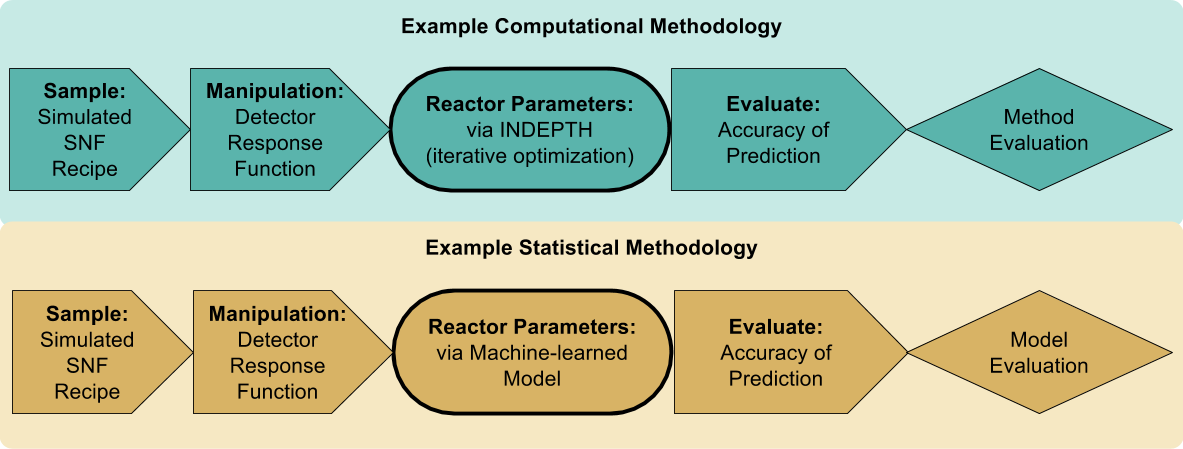
\includegraphics[width=\linewidth]{./chapters/intro/CompStatForensicsWorkflow.png}
  \caption{Diagram showing examples of forensics research using computational methodologies.}
  \label{fig:compworkflow}
\end{figure}

Because \gls{INDEPTH} is better studied and validated than statistical methods,
this work focuses on a statistical approach but with the intention to compare
methodologies.  Since focusing on rapid characterization is also a main goal, the
data input to the tool will be manipulated to reflect the information reduction
of a gamma detector measuring the \gls{SNM}. Thus, this work evaluates to what
degree statistical methods will be able to predict reactor parameters with
respect to the type of training data used.  

